\section{Results}
\label{sec:results}

\paragraph{Teacher Probe Results.}

The three teacher probes all reach high Mini-ImageNet accuracy on frozen VLM visual features, supported by the fact that the dataset was part of the original VLM pretraining.
This matters because the probes are saliency sources: a stronger or more complex probe is useful only if its gradients provide better distillation guidance.
Table~\ref{tab:probe-results} shows that the mean probe obtains the highest validation and test accuracy.

\begin{table}[H]
  \centering
  \caption{Teacher-probe results on frozen VLM visual features.}
  \label{tab:probe-results}
  \small
  \begin{tabular}{@{}lrrr@{}}
    \toprule
    Probe type & Best epoch & Val accuracy & Test accuracy  \\
    \midrule
    Mean & 10 & \textbf{95.07} & \textbf{95.00} \\
    Attention & 2 & 94.93 & 94.48 \\
    Cross-attn & 10 & 94.58 & 94.78 \\
    \bottomrule
  \end{tabular}
\end{table}


\paragraph{Generated-Answer Results.}

Table~\ref{tab:primary-results} reports the primary image-grounded preference results on a shared subset of 437 images, retaining an image only when all three judges produced valid preferences for every student variant, from the original 500 pool of images.
The teacher remains preferred for most images in every condition, so the current students should not be viewed as complete replacements for the original visual pathway.
The important comparison is between student variants.
Plain global reconstruction is weak: the baseline receives only 10 student-majority wins.
Every explanation-guided variant improves on this baseline, and the best variant, mean-probe explanation-only distillation, receives 69 student-majority wins.


\begin{table}[t]
  \centering
  \caption{LLM jury results}
  \label{tab:primary-results}
  \scriptsize
  \setlength{\tabcolsep}{2.2pt}
  \begin{tabular}{@{}lrrrrr@{}}
    \toprule
    Variant & Student & Teacher & Not Majority & All Agree &  $\kappa$ \\
    \midrule
    Base MSE & 10 & 427 & 0 & \textbf{0.936} &  0.312 \\
    Mean, loss expl. & \textbf{69} & 367 & 1 & 0.705 &  0.355 \\
    Attn, loss expl. & 56 & 381 & 0 & 0.741 &  0.367 \\
    Cross, loss expl. & 20 & 416 & 1 & 0.856 &  0.337 \\
    Mean, loss MSE+expl. & 58 & 379 & 0 & 0.737 &  0.355 \\
    Attn, loss MSE+expl. & 61 & 376 & 0 & 0.737 &  0.338 \\
    Cross, loss MSE+expl. & 37 & 400 & 0 & 0.817 &  \textbf{0.372} \\
    \bottomrule
  \end{tabular}
\end{table}

% \begin{figure}[t]
%   \centering
%   
\includegraphics[width=\linewidth]{figures/primary_preference_valid3}
%   \caption{Student preference rate on the shared valid image-grounded subset ($n=437$ for every variant). Counts above bars show student-majority wins. Explanation-guided distillation improves over the plain MSE baseline for every probe family.}
%   \label{fig:primary-results}
% \end{figure}

% Figure~\ref{fig:primary-results} makes the ablation clearer.
% The strongest explanation-only model outperforms both the baseline and its corresponding combined global-plus-explanation version.
% This suggests that saliency-weighted local matching is not merely a weak auxiliary regularizer.
% Figure~\ref{fig:combined-evidence}(a) reports the voting tendency of each judge.
% All judges prefer teacher answers on most images, but each shifts toward the mean explanation-only student relative to the global MSE baseline: the student-preference counts rise from 14 to 76 for Qwen3.5-9B, from 17 to 92 for GLM-4.6V-Flash, and from 10 to 78 for MiniCPM-V-4.5.
% Ties are nearly absent.

% \begin{figure*}[t]
%   \centering
%   
\includegraphics[width=\textwidth]{figures/judge_preference_tendencies_tufte}
%   \vspace{0.35em}
%   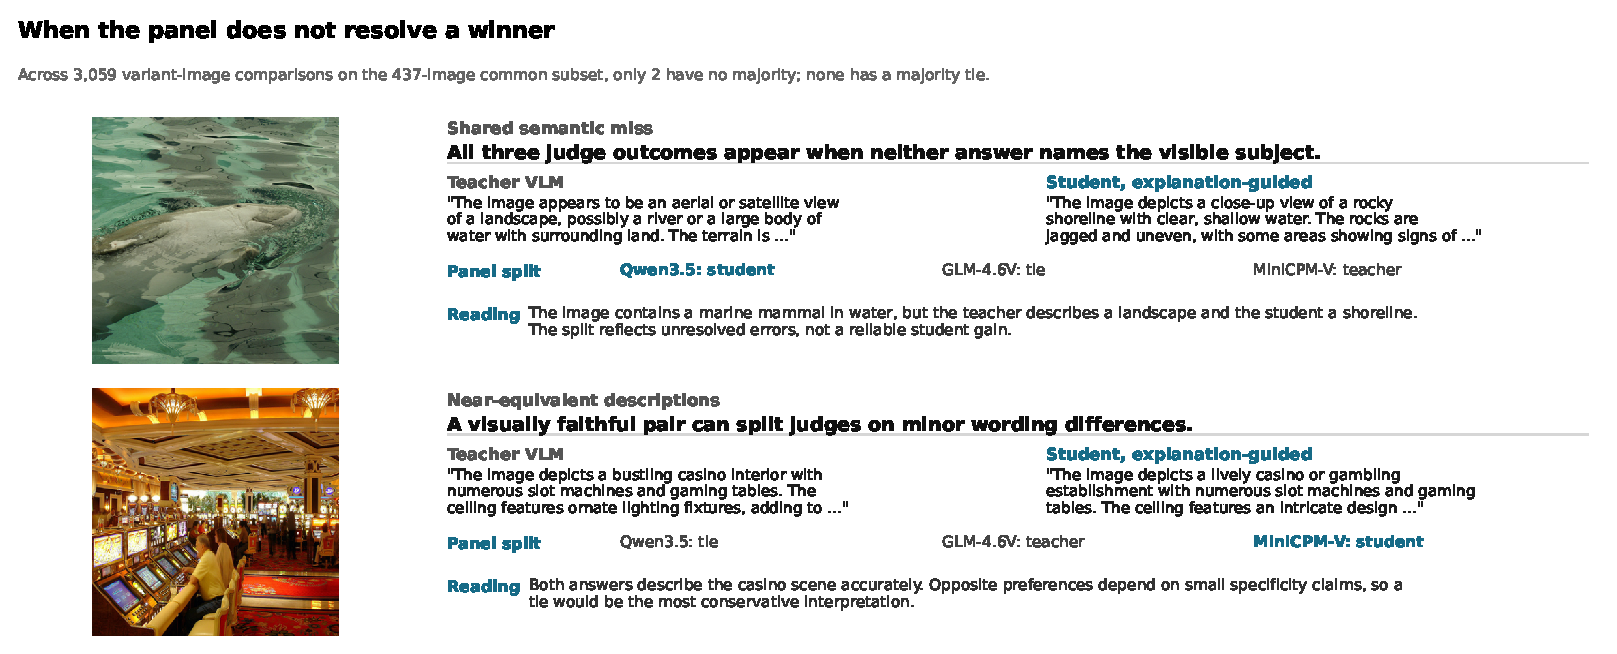
\includegraphics[width=\textwidth]{figures/qualitative_panel_splits}
%   \caption{Quantitative and qualitative evidence for the effect of explanation guidance. \textbf{(a)} Individual judge preferences on the shared valid subset ($n=437$ images per student variant): gray bars and left-hand counts indicate teacher preference, blue bars and right-hand counts indicate student preference, and the center column records ties. \textbf{(b)} The only two no-majority comparisons in that subset; direct judge labels expose three-way panel splits rather than majority ties. Panel (c) continues with representative answer patterns.}
%   \label{fig:combined-evidence}
% \end{figure*}

% \paragraph{Automatic Text Similarity}
% \label{sec:automatic-text-similarity}

% BERTScore provides a text-only diagnostic of semantic similarity between teacher and student answers.
% It is not the primary metric because it cannot verify visual faithfulness, but it helps show whether the student output remains linguistically close to the teacher.
% The same ordering appears only partially: the mean explanation-only model has the highest BERTScore F1, but the attention variants are nearly tied despite different image-grounded preference results.
% This gap reinforces the need for image-grounded evaluation.

% \begin{table}[t]
%   \centering
%   \caption{BERTScore diagnostics over generated teacher/student answers.}
%   \label{tab:bertscore}
%   \small
%   \begin{tabular}{@{}lccc@{}}
%     \toprule
%     Variant & Precision & Recall & F1 \\
%     \midrule
%     Base MSE & 0.891 & 0.881 & 0.886 \\
%     Mean expl. & 0.918 & 0.910 & 0.914 \\
%     Mean MSE+expl. & 0.916 & 0.908 & 0.912 \\
%     Attn expl. & 0.916 & 0.910 & 0.913 \\
%     Attn MSE+expl. & 0.916 & 0.909 & 0.913 \\
%     Cross expl. & 0.909 & 0.901 & 0.905 \\
%     Cross MSE+expl. & 0.909 & 0.902 & 0.906 \\
%     \bottomrule
%   \end{tabular}
% \end{table}

% \paragraph{Effect of the Saliency Source}
% \label{sec:effect-saliency-source}

% The choice of saliency source matters.
% Mean-probe explanations give the strongest explanation-only result.
% Attention-probe explanations are also competitive, especially when combined with global reconstruction.
% Cross-attention saliency is weaker in both objective settings.
% This pattern suggests that a more expressive probe does not automatically provide better distillation guidance.
% For explanation-guided distillation, the saliency source should be treated as part of the method rather than as a minor interchangeable choice.

% Agreement is highest for the baseline because judges almost always prefer the teacher.
% Thus, high agreement does not imply a better student.
% The more relevant signal is whether the student wins more often under blind image-grounded comparison.

\paragraph{Qualitative Analysis}
\label{sec:qualitative}

% To complement the aggregate preferences, the judged reports were inspected across the same 500 images used by all variants.
% This analysis is not intended as a separate benchmark; it is used to characterize what changes when the distillation objective is guided by saliency.
% Across the 500 shared test images, there are 59 cases in which the plain MSE baseline is not student-preferred while at least three of the six explanation-guided variants are student-preferred.
% In 8 cases, all six explanation-guided variants are student-preferred while the baseline is not.
% The reverse finding is equally important: in 350 cases, the teacher remains preferred over every student variant.
% Thus, explanation-guided distillation does not uniformly close the teacher-student gap.
% Its gains are concentrated in visually specific cases where the answer depends on preserving local evidence.
Figure~\ref{fig:qualitative-patterns} illustrates what changes in the generated answers when the student is trained with explanation guidance.
In the first two cases, the guided student preserves visible evidence that the global MSE baseline loses: it describes the texture of the mushroom cap more precisely and recognizes the bowls instead of inventing shoes. The lower two examples also show the limit of this result. For the Triceratops skull, the guided student identifies the main object but misses the person and wider scene context captured by the teacher. In the second skeleton example, explanation guidance prevents the severe baseline failure of claiming that no image is available, a problem observed when the distilled visual embeddings do not lie in the distribution expected by the language model. Taken together, these cases indicate improved visual grounding and robustness.


\begin{figure*}[t]
  \centering
  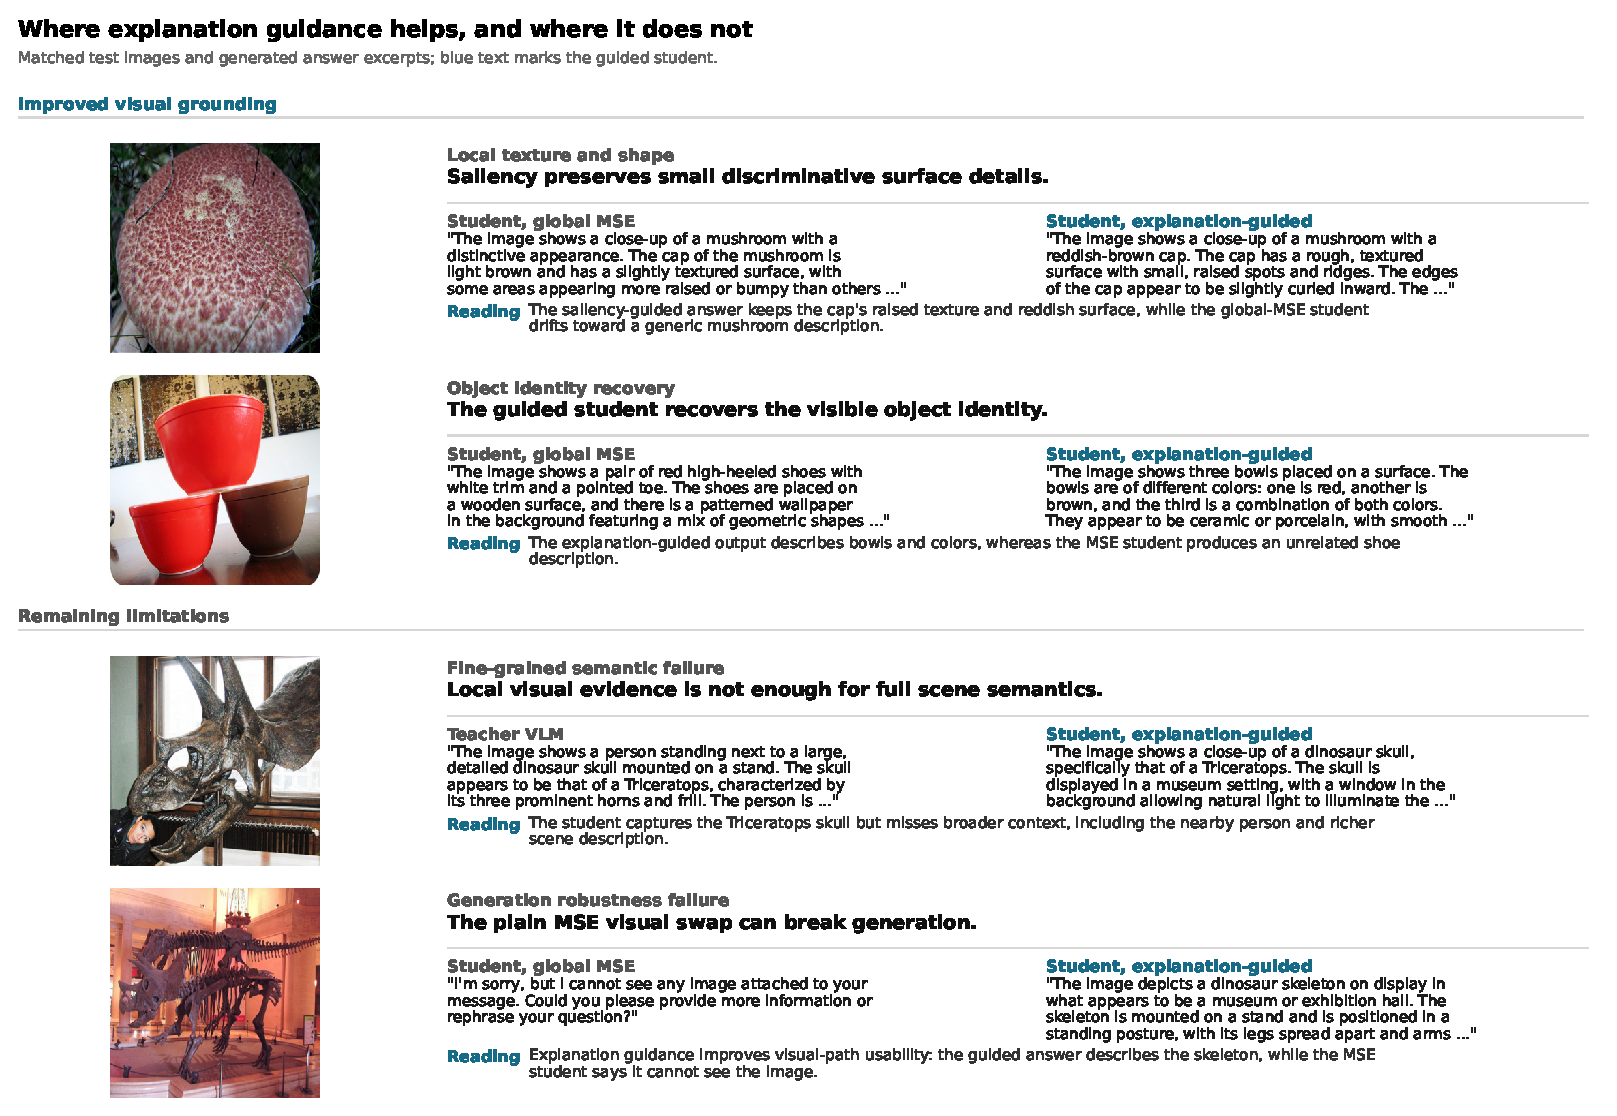
\includegraphics[width=\textwidth]{figures/qualitative_patterns_combined}
  \caption{Representative qualitative patterns in generated answers. The upper cases illustrate visual evidence preserved by explanation-guided distillation; the lower cases expose remaining limitations or baseline failure modes.}
  \label{fig:qualitative-patterns}
\end{figure*}

% \begin{table*}[t]
%   \centering
%   \caption{Qualitative patterns from the image-grounded judged reports. Source indices identify examples in the sampled test set.}
%   \label{tab:qualitative-patterns}
%   \small
%   \begin{tabular}{@{}p{0.21\textwidth}p{0.38\textwidth}p{0.33\textwidth}@{}}
%     \toprule
%     Pattern & Representative observation & Interpretation \\
%     \midrule
%     Local texture and shape &
%     In mushroom and coral examples (sources 4914 and 4854), explanation-guided students preserve cap texture, raised surface details, or rounded coral structure more faithfully than the baseline student. &
%     Saliency weighting helps when the decisive visual evidence is concentrated in local regions rather than in the global image embedding. \\
%     Object identity recovery &
%     In examples involving a marine mammal, an elongated green object, and stacked bowls or cups (sources 513, 436, and 3287), several explanation-guided variants recover the visible object while the baseline produces a refusal-style answer or an unrelated object. &
%     The explanation signal can stabilize object-level grounding after the visual module is swapped into the VLM. \\
%     Fine-grained semantic failures &
%     Dinosaur and triceratops examples (sources 111, 143, and 148) remain difficult: students often describe a generic skull, statue, or skeleton and miss the specific category, nearby person, or museum context. &
%     Saliency over visual tokens does not by itself provide all high-level semantic distinctions needed by the language model. \\
%     Generation robustness failures &
%     The plain MSE baseline produces 67 no-image or refusal-style student answers, while explanation-guided reports contain almost none of these failures. &
%     Some preference gains come from keeping the swapped visual path usable for generation, not only from making descriptions more detailed. \\
%     \bottomrule
%   \end{tabular}
% \end{table*}



\section{Limitations}
\label{sec:limitations}

This study evaluates one teacher VLM, one dataset, and one prompt family.
The conclusions should therefore be read as evidence that explanation-guided distillation is promising, not as a universal result across VLMs.
The judges are VLMs rather than human annotators, so their preferences may contain model-specific biases even under blind answer ordering.
The saliency signal is also mediated by a probe, which may emphasize class-discriminative evidence rather than every detail needed for open-ended generation.
Finally, the current students remain clearly below the teacher in absolute preference, which means the method improves replacement fidelity but does not yet solve faithful visual-module substitution.

\section{Conclusion}
\label{sec:conclusion}

We studied whether explanations can guide knowledge distillation for a VLM visual module.
The student ViT is trained using Grad-CAM-weighted token reconstruction and then plugged into the original VLM so that evaluation happens through generated answers.
Across all tested saliency sources, explanation-guided objectives outperform plain global MSE under image-grounded blind judging.
The strongest result comes from explanation-only supervision, suggesting that explanations can provide a meaningful distillation signal rather than only a secondary regularizer.
Future work should test richer prompts, human preference labels, stronger student adapters, and saliency objectives aligned more directly with the multimodal representation consumed by the language model.
